\documentclass[conference]{IEEEtran}
\IEEEoverridecommandlockouts

\usepackage{cite,amsmath,amssymb,graphicx,booktabs,url}
\usepackage[hidelinks]{hyperref}
\hypersetup{
  pdftitle={Tact: A Zero-Cost, Browser-Based Pipeline for On-Demand Tactile Braille Storybooks},
  pdfauthor={Iliano Fasolino},
  pdfsubject={Accessible on-demand tactile Braille storybooks via a zero-cost browser pipeline with graceful degradation},
  pdfkeywords={Braille, tactile graphics, accessibility, assistive technology, blind children, Braille literacy, 3D printing, fused deposition modeling, in-browser LLM, WebGPU, human-computer interaction}
}

\graphicspath{{figures/}}

\begin{document}

\title{Tact: A Zero-Cost, Browser-Based Pipeline for On-Demand Tactile Braille Storybooks}

\author{\IEEEauthorblockN{Iliano Fasolino}
\IEEEauthorblockA{Independent Researcher\\
Milan, Italy}}

\maketitle

\begin{abstract}
Braille literacy among blind school-age children fell from roughly 50 percent in 1960 to under 10 percent today, and the decline is a content problem, not a technology problem: producing one illustrated Braille page still requires specialized software and trained labor, so almost nothing in the existing catalog is personalized to an individual child. We present Tact, a system that converts a spoken or typed story idea into a printable Braille page with a matching raised tactile illustration, computed inside a web browser with no account and no mandatory cost, and able to run with no server at all. This paper documents the full engineering history behind that system, rather than a narrow slice of it. It covers the target population and the ethical framing behind an explicit sighted-operator model, the hardware rationale for desktop fused deposition modeling over purpose-built embossing, and the physical Braille geometry and its printer-specific calibration. It documents the architecture that lets a language model run on the reader's own device, the later addition of a faster hosted path in front of it after an independent reimplementation exposed the cost of a 1.8 gigabyte first-use download, and the fallback chain that keeps the system working when that path is absent, the investigation that replaced a general-purpose Braille translation library with a small deterministic implementation after it failed in production, and the evolution of the page layout from an inherited portrait specification to a verified square design. It further documents the construction of an 89-shape hand-drawn tactile illustration library derived from a frequency study of fairy-tale subjects, and the synthesized sound design used to make a voice-first interface legible without a screen. We report the verification performed to date, the ethical commitments the project has made, and the work required before the system can be considered ready for real blind and low-vision readers.
\end{abstract}

\section{Introduction}\label{sec:intro}

A sighted five-year-old who asks for a story about a dragon afraid of the dark can have one within minutes. A parent invents it, or a book already sitting on the shelf supplies one among dozens of alternatives. A blind five-year-old asking for the same story has, in practice, no equivalent option. Braille transcription of a single page has historically required a trained transcriber and specialized software, particularly when the page includes a tactile illustration, and the specialist labor involved has never scaled the way print production scaled. The catalog of Braille children's books is, as a result, a small fraction of what exists in print, and it contains almost nothing personalized to an individual child's own obsessions, pets, or worries.

The consequence is measurable rather than anecdotal. Braille literacy among legally blind school-age children in the United States fell from approximately 50 percent in 1960 to roughly 8.5 percent today \cite{nfb2024}, illustrated in Fig.~\ref{fig:literacy}. Over half of blind students currently enrolled in public education are identified as non-readers or pre-readers of Braille. Ninety percent of employed blind adults are Braille literate, while only one in three adults who do not know Braille is employed \cite{nfb2024}. These two facts are connected. Audio tools such as screen readers and audiobooks are effective for consumption, but they do not build the same relationship with written language that decoding text under one's own fingers builds. A person who has only ever been read to has a fundamentally different relationship with language than a person who has decoded it themselves, letter by letter. This distinction between literacy and consumption motivates the present work.

\begin{figure}[t]
\centering
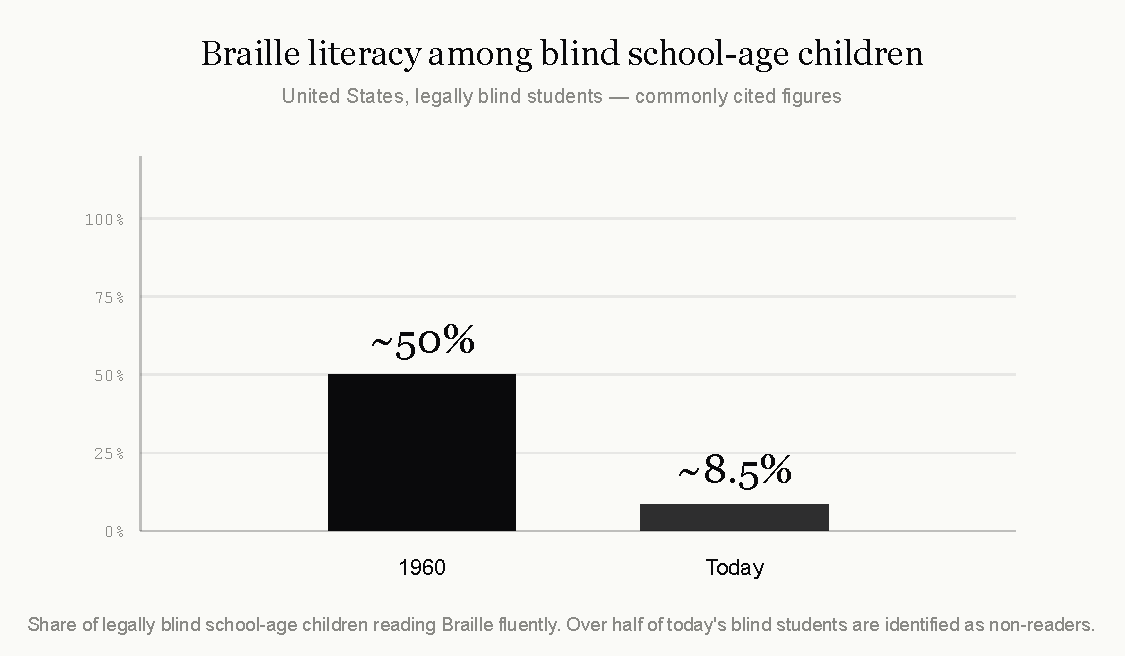
\includegraphics[width=\columnwidth]{chart-literacy.pdf}
\caption{Braille literacy among legally blind school-age children in the United States, 1960 versus today. The decline from roughly 50 percent to roughly 8.5 percent tracks closely with the mainstreaming of blind children into public schools after the Rehabilitation Act of 1973, which reduced the density of Braille-qualified teachers per student \cite{nfb2024}.}
\label{fig:literacy}
\end{figure}

The historical turning point behind the decline is well documented. The Rehabilitation Act of 1973 moved large numbers of blind children out of specialized schools for the blind and into mainstream public schools, where the density of Braille-qualified teachers per student fell sharply, because most public schools could not justify hiring and training a dedicated Braille instructor for a small number of students. Italy follows a structurally similar pattern: the \emph{insegnante di sostegno} mainstreaming model reduces the amount of dedicated Braille instruction time a blind child receives relative to a specialized institute. The mechanism differs by country, but the outcome, a widening gap between the number of blind children and the number of adults qualified to teach them Braille, recurs internationally.

This paper documents Tact, a system built to address the content half of that gap rather than the teacher-supply half, which is a separate and harder policy problem outside this paper's scope. Tact converts a one-sentence spoken or typed story idea into a finished, printable Braille page with a matching raised tactile illustration, computed entirely inside a web browser tab. Sections~\ref{sec:related} through~\ref{sec:conclusion} document, in order, the related systems this work builds on and departs from, the target population and the ethical framing behind that choice, and the formal requirements the project treats as non-negotiable. They then cover the hardware rationale, the full system architecture, and five detailed engineering case studies drawn directly from the project's own build history. The remaining sections report the physical fabrication calibration data, the sound design system, a set of representative use cases, the verification performed to date, and the limitations that remain before any claim of readiness for real readers.

\section{Related Work}\label{sec:related}

Several existing systems address parts of the problem Tact targets, and each informed a specific design decision documented later in this paper.

Liblouis is an open-source Braille translation engine covering roughly 150 language tables, used inside screen readers including NVDA and JAWS \cite{liblouis}. It is the correct default instinct for Braille translation, and Section~\ref{sec:braille} documents why it was nonetheless replaced for this project's in-browser deployment after a direct engineering investigation.

BrailleRAP is an open-source, self-buildable Braille embosser, certified as open hardware and costing roughly 250 to 350 euros in parts \cite{braillerap}. A closely related project, Tactipix, uses BrailleRAP hardware to produce illustrated children's books with audio, in which illustrations can be embossed alongside text. Tactipix is the closest existing sibling to Tact in spirit. It is not automated, and it is tied to a single piece of do-it-yourself hardware rather than to widely available consumer 3D printers. Section~\ref{sec:hardware} details the hardware rationale that led Tact toward fused deposition modeling instead.

TaleVision combines multimodal artificial intelligence with real-time tactile and auditory feedback to help blind children connect Braille and imagery, and it was evaluated directly with children with congenital visual impairment \cite{talevision}. This is the closest published academic validation of the underlying concept, and it demonstrates that AI-assisted tactile content genuinely improves outcomes for blind children in a controlled study. It is, however, a research prototype rather than an open, deployable system a parent or school can install today.

TactileNet contributes a large, purpose-built dataset for training models to generate tactile graphics \cite{tactilenet}. It is a dataset, not a deployable end-user tool, but its existence supports the premise, adopted directly in this project's own shape library design (Section~\ref{sec:illustration}), that tactile-graphic generation should draw on curated, tactilely legible shape sets rather than on traced photographs or unmodified clip art.

AltCanvas offers a tile-based editor through which a blind or low-vision user manually assembles a tactile scene with generative-AI assistance \cite{altcanvas}. It is a manual composition tool built for an adult or a trained professional. Tact instead composes the page automatically from a one-sentence prompt, trading manual creative control for a near-zero operating burden appropriate for a busy parent.

Chart4Blind converts bitmap data charts into accessible vector graphics for sighted authors preparing material for blind readers \cite{chart4blind}. It is domain-specific to charts rather than general narrative illustration, but its end-to-end accessible-SVG pipeline is a useful architectural reference.

tactile-svgdreamer is a research pipeline that generates tactile-optimized SVGs directly from text prompts, and it is useful as a reference for what a tactile-optimized SVG should visually resemble. It requires a CUDA-capable graphics processing unit for inference, which rules it out entirely for a project whose first requirement (Section~\ref{sec:requirements}) is that no step depend on a dedicated GPU.

Table~\ref{tab:relatedwork} summarizes how each related system compares to Tact along the dimensions that matter most: automation, deployability, hardware dependency, and personalization.

\begin{table}[t]
\caption{Comparison of Tact against the closest related systems.}
\label{tab:relatedwork}
\centering
\begin{tabular}{lccc}
\toprule
System & Deployable today & No GPU needed & Automated \\
\midrule
Liblouis \cite{liblouis} & Yes (library) & Yes & N/A \\
BrailleRAP \cite{braillerap} & Yes & Yes & No \\
TaleVision \cite{talevision} & No & Unknown & Partial \\
TactileNet \cite{tactilenet} & No (dataset) & N/A & N/A \\
AltCanvas \cite{altcanvas} & Yes & Unknown & No (manual) \\
Chart4Blind \cite{chart4blind} & Yes & Unknown & Chart-only \\
Tact (this work) & Yes & Yes & Yes \\
\bottomrule
\end{tabular}
\end{table}

None of these systems combines on-demand personalized story generation, automatic Braille translation, and automatic tactile illustration in one tool a non-specialist can operate without an account or a bill. None targets hardware a family is likely to already own. Tact is built to close that specific combination of gaps. Its contribution is not a single novel algorithm. It is an integrated, zero-cost pipeline, together with the engineering decisions, verified against real device constraints and documented in Sections~\ref{sec:llm} through~\ref{sec:illustration}, that make such a pipeline function reliably in an ordinary browser tab.

\section{Target Population and Ethical Framing}\label{sec:population}

\subsection{Primary and Secondary Users}

The primary users are blind and low-vision children roughly aged four to ten, spanning the developmental window during which fluent Braille acquisition happens most naturally. This window parallels the window in which sighted children acquire fluent print literacy, and evidence from Braille education research indicates that waiting past it measurably increases the difficulty of building fluent tactile reading later.

The secondary users are deafblind children and adults, for whom Braille is frequently the only literacy channel available at all. Audio alternatives that serve blind-but-hearing users are not an option for this population, which makes the zero-audio-dependency requirement discussed in Section~\ref{sec:requirements} directly relevant rather than a hypothetical edge case. The primary Italian point of contact for the deafblind population is Lega del Filo d'Oro, based in Osimo, in the Marche region, which the project intends to approach directly once a testable version exists.

\subsection{Explicit Scope Boundaries}

The system is deliberately not targeted at deaf users, who have full visual access to print and are already well served by existing tools, nor at blind adults, who have generally settled into an audio- and screen-reader-centric workflow this project has no interest in disrupting. Scoping a tool tightly is itself a design decision. A system that tries to serve every population with a stake in accessibility tends to serve the population with the most urgent, narrow need, young blind children inside the literacy-acquisition window, worse than a system built for them specifically.

\subsection{The Operator Model}

Tact assumes a sighted operator, a parent, teacher, or caregiver, who runs the software and the three-dimensional printer, while the blind child is the reader. This is stated explicitly rather than treated as a compromise to be hidden. The printer is conceived as a shared household or classroom appliance, not a device the blind user is expected to operate solo, and the software interface is nonetheless built to be fully screen-reader-accessible and voice-first, because the same child who reads a printed page today may be the one requesting tomorrow's story.

\subsection{Nothing About Us Without Us}

Every design choice documented in this paper was made by a sighted developer working from published research and standards, not from lived experience of blindness. The project treats that fact as a real limitation, not a footnote, following a principle common in disability-rights organizing: decisions affecting a community should not be finalized without members of that community. Direct contact with blind and deafblind users, and with the organizations that represent them, is treated as a hard prerequisite before any version of this tool is described as ready. The organizations named for this purpose are the Biblioteca Italiana per i Ciechi Regina Margherita in Monza, the Istituto dei Ciechi di Milano, UICI Lombardia, and Lega del Filo d'Oro. It is not an optional step to be added after a soft launch, and it has not yet occurred, a limitation restated explicitly in Section~\ref{sec:limitations} and revisited alongside two further ethical commitments in Section~\ref{sec:ethics}.

\section{Design Requirements}\label{sec:requirements}

The system was built against a short list of requirements treated as non-negotiable throughout development, the kind of list a team writes once, early, specifically so that later convenience never quietly erodes it.

\begin{enumerate}
\item \textbf{No graphics processing unit required for the baseline experience.} Braille translation, page layout, illustration matching, and stereolithography (STL) export must all function on a device with no dedicated graphics hardware whatsoever. A capable graphics processing unit may improve the experience through better AI-written stories, but it must never be a precondition for a working one.
\item \textbf{No mandatory payment anywhere in the pipeline.} Every step, speech recognition, story writing, Braille translation, illustration, and three-dimensional export, must have a free path with no artificial ceiling, enumerated in full in Section~\ref{sec:zerocost}.
\item \textbf{Permissive licensing.} The project is released under the MIT license specifically so that schools, libraries, and nonprofit organizations can adopt, fork, and redistribute it without legal friction.
\item \textbf{Bilingual from the first commit.} Italian and English are both first-class languages, not a default language with a translation added afterward, reflecting both the developer's own context in Milan and the intent to be useful internationally from day one.
\item \textbf{Standards-compliant Braille geometry, always.} Every physical dimension follows ISO 17049:2013 \cite{iso17049}, with no shortcut permitted that trades tactile legibility for convenience.
\item \textbf{Hardware-agnostic output.} STL is the primary export target because fused deposition modeling printers are the most widely available fabrication devices, but the architecture does not hard-code an assumption that FDM is the only future output format.
\end{enumerate}

\section{Hardware Rationale}\label{sec:hardware}

The most consequential early decision was rejecting the more conventional hardware target, a purpose-built Braille embosser, in favor of consumer fused deposition modeling (FDM) three-dimensional printing. Table~\ref{tab:hardware} summarizes the comparison against BrailleRAP, the most directly comparable open embossing project \cite{braillerap}.

\begin{table}[t]
\caption{FDM three-dimensional printing versus BrailleRAP-style embossing.}
\label{tab:hardware}
\centering
\begin{tabular}{lll}
\toprule
Factor & FDM printing & BrailleRAP embossing \\
\midrule
Acquisition cost & 50--100 EUR & 250--350 EUR (parts) \\
Output durability & High (years) & Low (paper wears) \\
True 3D relief & Yes & No (2.5D only) \\
Material cost & Low, rPET viable & Paper only \\
Operator skill & Low & Moderate \\
Device generality & Multi-purpose & Single purpose \\
\bottomrule
\end{tabular}
\end{table}

The print-time cost of FDM, minutes to a few hours per page, against seconds for embossing, was judged acceptable specifically because the intended output is a durable, re-read artifact a child keeps and returns to dozens of times, not a disposable bulletin. A slower process that produces something surviving years of handling was judged preferable to a faster process producing something that degrades within weeks. Thermoplastic polyurethane (TPU) at 95A hardness is the default material recommendation, because it best reproduces the flexibility of a paper page while surviving years of bending. Polyethylene terephthalate glycol (PETG) is offered as a rigid, washable alternative. Polylactic acid (PLA) is excluded from end-user recommendations due to brittleness, and recycled polyethylene terephthalate (rPET) is documented as a near-zero-cost option for cost-sensitive deployments, aligning the project with a circular-economy framing in addition to an accessibility one.

\section{System Architecture}\label{sec:architecture}

Tact runs as a single self-contained web application with no backend server. A parent, teacher, or child speaks or types a one-sentence story idea, and the remainder of the pipeline executes automatically. Story text is produced, split into balanced pages, translated into Grade 1 Braille, and matched to a tactile illustration. The result is laid out on a shared millimeter coordinate system and rendered both as an on-screen preview, styled following the typographic principles in Section~\ref{sec:visual} and accompanied by the synthesized feedback described in Section~\ref{sec:sound}, and as a binary STL file, ready for an FDM three-dimensional printer. Fig.~\ref{fig:pipeline} shows the full pipeline as implemented, from input capture through to printer output.

\begin{figure*}[t]
\centering
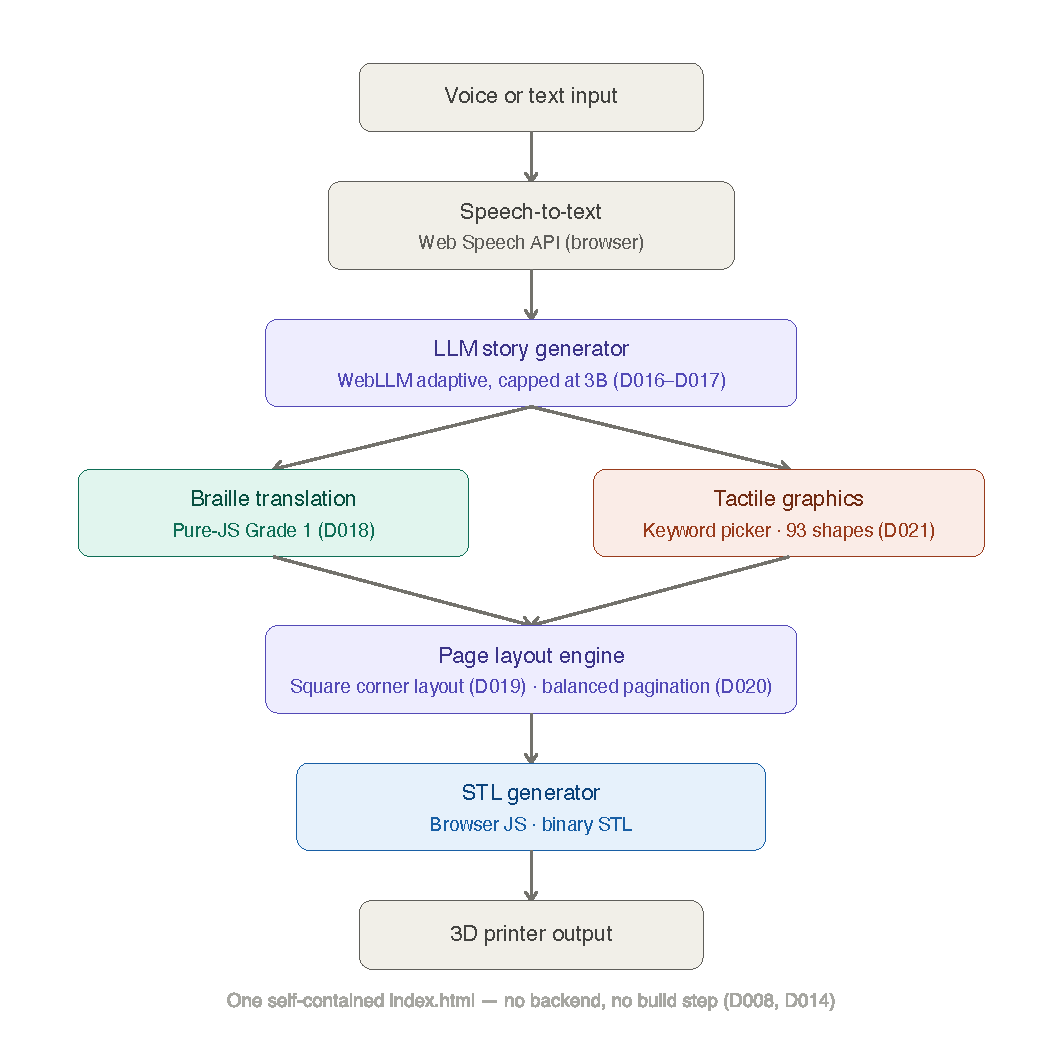
\includegraphics[width=0.72\textwidth]{tact_pipeline_architecture.pdf}
\caption{The complete Tact pipeline, running inside a single \texttt{index.html} file, with story writing supplied by a hosted model, an in-browser model, or the reader's own words, in that order of preference. Voice or typed input is transcribed by the browser's native speech recognition, passed to an adaptively sized in-browser language model (Section~\ref{sec:llm}), and then split into a Braille translation path (Section~\ref{sec:braille}) and a tactile graphics path (Section~\ref{sec:illustration}) that execute in parallel before being merged by the page layout engine (Section~\ref{sec:layout}) and exported by the binary STL generator (Section~\ref{sec:fabrication}).}
\label{fig:pipeline}
\end{figure*}

An early design phase specified a strict structured data contract between story generation and every downstream module, expressed as a nested object containing, at the top level, a language code, a Braille grade, a title, a URL-safe slug, a layout identifier, and an ordered array of pages. Each page carried plain story text, capped at approximately 20 words for the default layout, together with an optional illustration specification containing a scene description, a layout hint, and one to four typed illustration elements, each naming a shape from the library, a scale factor, a position hint, and a mirroring flag. This contract was intended to let any capable backend, a locally run large model, a cloud API, or an in-browser model, plug into the same downstream Braille translation, illustration matching, layout, and export logic without modification. Section~\ref{sec:llm} documents why the browser's default in-browser model does not, in practice, use this schema directly, and what replaced it for that specific path while preserving the schema as the target contract for more capable backends.

The single-file, no-backend architecture was chosen over a more conventional client-server split for a reason tied directly to the zero-cost requirement in Section~\ref{sec:requirements}. A server, however cheap, is a recurring bill and a single point of failure that can be discontinued, and an account system is a barrier a stressed parent at nine in the evening should never have to clear. A file that opens directly from local disk or from any static host and runs the entire pipeline locally has no such failure mode, and it can be copied to a portable storage device and handed to a school with no connectivity story required at all.

\section{Case Study: In-Browser Language Model Inference}\label{sec:llm}

\subsection{Why the First Version Refused a Remote Server}

A cloud-hosted language model is the most obvious way to obtain consistently well-written stories. It was rejected as the default path for three compounding reasons rather than one. It reintroduces a recurring cost that violates the zero-cost requirement the moment usage exceeds whatever a developer is willing to subsidize indefinitely. It requires an application programming interface (API) key, which reintroduces an account and setup barrier. It also means every story a family generates passes through a third-party server, an unnecessary privacy cost for content that is frequently about a specific, identifiable child.

The alternative adopted instead loads a small language model directly into the browser tab, over the WebGPU application programming interface \cite{w3cwebgpu}, and runs inference entirely on the visitor's own hardware, following the architecture described for the WebLLM in-browser inference engine \cite{webllm}. Nothing leaves the device during story generation, and there is no server-side compute to bill for.

That reasoning was sound on privacy and cost, and it remains the reasoning behind the path the system still ships. It was, however, incomplete on one axis the authors weighted too lightly, and Section~\ref{sec:hosted} documents what a second implementation of this system revealed about it.

\subsection{What an Independent Reimplementation Exposed}\label{sec:hosted}

Shortly after the first public version of this work was released, Francesco Giuliani independently rebuilt it as a production web application, published as \emph{tatto.dev} \cite{tattodev}. That reimplementation replaced the in-browser model with a hosted one reached through a server route, reduced the JavaScript payload by roughly 94 percent, moved the codebase to TypeScript with unit tests on the Braille tables, and corrected a defect in which selecting Italian still produced English stories. The two projects share no code and evolve independently.

The substantive contribution of that work to this one is not an implementation detail but a correction to the argument above. The in-browser design was defended as the choice that imposed no barrier on anyone. In practice it imposes a very specific and very large one: a first-use model download of roughly 1.8 gigabytes. For the households and schools this project explicitly targets, which are disproportionately those on slow, metered, or shared connections, that download is a heavier barrier than the account it was meant to avoid. It also excludes mobile devices almost entirely. The original analysis had correctly identified the costs of a server while systematically underweighting the cost of the alternative.

The system was therefore restructured, not by removing the in-browser path but by placing a faster one in front of it. Story generation now attempts three paths in order. A hosted model is tried first, reached through a minimal proxy described below. If that path is unavailable, rate limited, or removed entirely, the in-browser model of Section~\ref{sec:llm} runs exactly as before. If the device cannot run that either, the reader's own words become the printed page. Every claim of graceful degradation made in the first version survives intact, because the paths beneath the new one were not modified.

\subsection{Holding a Key Without Holding a Server}

A hosted model requires authentication, and a static page cannot hold a secret. Placing an API key in client-side JavaScript would publish it to anyone who opened the developer tools. The system therefore introduces exactly one server-side component, a proxy of roughly 150 lines deployed on a serverless platform, whose only responsibilities are to hold the key, to accept a one-line story idea, and to return prose.

Two properties of that proxy are deliberate. The story brief lives inside the proxy rather than travelling in the request, so a caller who discovers the endpoint can obtain a children's story and nothing else; the endpoint cannot be repurposed as a general-purpose language model. Requests are additionally restricted to the project's own origins. The proxy stores nothing, and no account exists at any layer.

This is a genuine change to the system's privacy posture and is stated plainly rather than minimized. On the hosted path, the one-line idea a child or adult supplies leaves the device and reaches a third party. Nothing else is transmitted, but that sentence is. The in-browser path continues to transmit nothing at all, and remains available by removing the proxy endpoint from the configuration, which disables the hosted path entirely and returns the system to its original behavior. The honest formulation of the resulting claim is not that the system runs without a server, but that it \emph{works} without one, and that the hosted path is an accelerator rather than a dependency.

\subsection{Measured Effect of the Hosted Path}

The hosted path uses \texttt{agnes-2.0-flash}, an OpenAI-compatible model offered without charge at the time of writing \cite{agnes}. Its free tier carries no stated expiry, which is a commercial position rather than a guarantee, and the fallback chain exists partly because that position may change.

Table~\ref{tab:hosted} reports the effect measured over approximately 150 generated stories. The comparison of interest is not raw inference speed but time-to-first-story on a device that has never visited the site before, which is the only figure a family or a classroom actually experiences.

\begin{table}[t]
\caption{Time to a printable page on a first visit, by generation path}
\label{tab:hosted}
\centering
\begin{tabular}{@{}lrr@{}}
\toprule
\textbf{Path} & \textbf{First visit} & \textbf{Transfer} \\
\midrule
In-browser model (3B tier) & several minutes & $\approx$1.8\,GB \\
Hosted model via proxy & 6.3--9.2\,s & $<$2\,kB \\
Reader's own words & $<$1\,s & none \\
\bottomrule
\end{tabular}
\end{table}

Request success was measured separately, since a free tier implies a rate ceiling. At up to eight concurrent requests, 31 of 32 succeeded, the single failure being a client-side timeout rather than a rejection. Under a deliberately abusive burst of 40 requests issued as fast as the network allowed, 15 were rejected as rate limited. Sequential use at approximately five requests per minute produced no rejections at all. The practical reading is that ordinary use does not reach the ceiling, that a sudden surge of attention will, and that the fallback chain is what makes the second case a slower story rather than no story.

\subsection{Adaptive Model Selection and a False Positive Worth Documenting}

Not every device can run the same size of model. The system profiles the browser's WebGPU adapter at runtime and walks down a tier list from largest to smallest, falling back automatically to the next smaller tier if a given model fails to initialize. Table~\ref{tab:tiers} lists the tier list actually shipped.

\begin{table}[t]
\caption{Adaptive language model tier list, largest to smallest.}
\label{tab:tiers}
\centering
\begin{tabular}{lrr}
\toprule
Tier & Approx. VRAM & Approx. download \\
\midrule
8B (manual opt-in only) & 4.6 GB & 3.5 GB \\
3B (alternate family) & 2.5 GB & 2.0 GB \\
3B (\textbf{default ceiling}) & 2.3 GB & 1.8 GB \\
2B & 1.6 GB & 1.3 GB \\
1B & 0.9 GB & 0.7 GB \\
\bottomrule
\end{tabular}
\end{table}

A genuinely counter-intuitive finding surfaced while building the selection logic. The browser's own capability signals cannot be trusted to identify a device as capable of running the largest tier. An ordinary laptop with no discrete graphics processing unit was observed, during development, to report a WebGPU adapter buffer size of exactly 4096 megabytes and a \texttt{navigator.deviceMemory} value of 8. A naive selection rule would read both signals as evidence of a capable device. They are common platform defaults rather than genuine capability indicators; the \texttt{deviceMemory} property is deliberately capped at 8 for privacy reasons regardless of a device's true installed memory, and 4096 megabytes is a frequent graphics driver default rather than a measurement of available memory. Treating these signals as genuine would route large numbers of ordinary laptops into a multi-gigabyte download that subsequently fails to initialize, wasting the visitor's time and bandwidth for nothing. The resolution adopted was to cap automatic selection deliberately at the three-billion-parameter tier, a substantial quality jump over the smallest model that still reliably runs on the large majority of WebGPU-capable devices. An eight-billion-parameter tier remains available, but only behind an explicit, informed, manual choice, never inferred automatically from these two signals.

\subsection{From a Structured Schema to Prose}

The original design, described in Section~\ref{sec:architecture}, called for the model to return the full structured object in a single call, including the typed illustration specification. In practice, the smallest usable in-browser model reliably failed to honor that contract. It wrote perfectly reasonable prose but ignored field-level constraints, and it placed descriptive sentences into fields meant to hold a single shape name. Output was frequently truncated well before the closing brace of the object, so the parser rejected the response outright. The pipeline fell back to a fixed demonstration story on nearly every request, silently defeating the entire point of the feature.

The fix was to stop fighting the model's actual observed behavior and instead request only what it is reliably good at: plain story text, nothing else. Pagination (Section~\ref{sec:layout}) and illustration-shape selection (Section~\ref{sec:illustration}) were moved out of the model call entirely and implemented as ordinary, deterministic, inspectable client-side logic. This is a case in which a design intended for a more capable backend had to be pragmatically adapted to the empirically observed behavior of the model shipping in the default configuration. The resulting text-only prompt is now the default even for larger, more capable models, because the simplification carried no measurable quality cost and a substantial reliability gain.

The prompt given to the model was rewritten with the target reader specifically in mind, rather than treated as a generic instruction to write a children's story. Because the reader experiences the story by touch rather than sight, the system prompt explicitly requests sensory language that favors touch, sound, warmth, and movement over color and visual description. It asks for a clear three-beat arc: a calm beginning, one small wish or problem, and a warm resolution. It permits gentle rhythm and soft repetition of a phrase, and it includes one hand-written example passage the model can pattern-match against for tone.

\subsection{Measured Effect of the Model Size and Prompt Changes}

The same prompt, a cat living on a boat on the moon, was run against both the smallest model tier with a generic prompt and the default three-billion-parameter tier with the rewritten sensory prompt, and both outputs were captured directly for comparison.

Before, using the one-billion-parameter tier and a generic prompt, the model produced: ``A black cat sat on the moon's surface. She felt the warm sun on her fur. The cat sat on the boat in the distance. The moon was her home.''

After, using the three-billion-parameter tier and the rewritten sensory prompt, the model produced: ``The soft fur of my cat friend felt the gentle rocking of the moon boat. I wish the stars would twinkle a little brighter, she thought. The warm sunbeams dancing on her whiskers made her feel cozy. As the boat glided over the craters, the sound of waves lapping against the hull soothed her. The scent of space dust and moonflowers filled the air. In the silence, she felt a gentle peace settle over her.''

The second passage is not merely longer. It is built almost entirely from touch, sound, warmth, and motion, fur, rocking, whiskers, lapping, scent, silence, which is precisely the vocabulary a reader experiencing the story through fingertips rather than eyes needs, and precisely what the prompt was rewritten to elicit rather than leaving to chance.

\subsection{Graceful Degradation Without a Demonstration Trap}

If the hosted path of Section~\ref{sec:hosted} is unavailable and the visitor's device has no WebGPU support either, or if model initialization fails for any reason, the system does not substitute a fixed demonstration story and call the interaction complete. The words the person actually typed or spoke are paginated using the same balancing logic described in Section~\ref{sec:layout}, translated to real Braille, matched to a real illustration by keyword, and exported to a real, printable STL file. A fixed demonstration is used only as a last resort, reached solely if every other step in the chain fails outright. Every visitor, regardless of hardware, leaves with a working product; the language model is a genuine enhancement, never a load-bearing dependency.

\section{Case Study: Braille Translation Engineering}\label{sec:braille}

\subsection{The Original Plan}

Braille translation was originally scoped around Liblouis, compiled to WebAssembly for in-browser use \cite{liblouis}. This was the correct default instinct. Liblouis is mature, standards-aligned, and not something to casually reinvent, and it remains the reference implementation this project's future locally installable package is expected to use.

\subsection{A Root-Cause Investigation}

In practice, the specific WebAssembly build of Liblouis available for browser deployment turned out to be unusable for this project, for three compounding reasons discovered through direct testing rather than assumed in advance. First, the bundled Unified English Braille (UEB) Grade 1 table failed to compile inside that particular WebAssembly build, because it referenced an opcode the build did not support, so every translation call for English silently returned a null result rather than raising a visible error \cite{ueb}. Second, several alternative English tables did not merely fail gracefully; they triggered a hard abort inside the WebAssembly heap, corrupting the module for every subsequent call within that session. Third, and most seriously, the application code that received a null translation result passed that null value into a Unicode-decoding routine, which threw an exception inside a worker thread's message handler. The pending JavaScript promise the rest of the application was awaiting therefore never resolved and never rejected. The visible symptom was not an error message. It was the entire application hanging indefinitely on a translating-to-Braille loading screen, with no feedback whatsoever to the person waiting.

\subsection{The Pivot}

Rather than continue debugging that specific WebAssembly build, the translation layer was rewritten from scratch as a small, pure-JavaScript character-to-cell mapping, and this turned out to be the more correct engineering choice for this project specifically, not merely a workaround forced by circumstance. Grade 1 Braille, the standard this project uses exclusively for both Italian and English, is by definition an uncontracted, one-character-to-one-cell mapping with no contextual ambiguity. A deterministic lookup table is not a simplified approximation of Grade 1 Braille; it is an exact implementation of it. The replacement is instant, has no external dependency, works fully offline and even from a local file with no network connection at all, and removed roughly 1.6 megabytes of WebAssembly download that was never functioning correctly in the first place.

\subsection{Why Grade 1 Is the Right Default, Not a Limitation}

Italian Braille has no Grade 2, contracted, form at all. Grade 1 is simply what Italian Braille is, governed by the Biblioteca Italiana per i Ciechi Regina Margherita in Monza. English defaults to Unified English Braille Grade 1 specifically because the target reader is a beginner \cite{ueb}. Grade 2's roughly 180 contractions are a skill introduced after Grade 1 fluency is established, not before it, so defaulting to Grade 1 is the developmentally correct choice for this audience rather than a reduced feature set adopted for convenience.

\section{Case Study: Page Geometry and Layout Engineering}\label{sec:layout}

\subsection{Coordinate System}

Every physical dimension in the system is expressed in millimeters. The coordinate system places its origin at the bottom-left of the page, with the Z axis increasing away from the print bed toward the reader's fingers. This convention was chosen specifically to match the coordinate convention three-dimensional printing slicers already use, which eliminates an entire class of vertical-axis-flip bugs between the design representation and the exported file.

\subsection{An Honest Account of a Layout That Changed Twice}

The original specification defined three selectable page layouts of increasing density: a picture-book layout with a short text block over a full-width illustration, a two-card layout separating text from a reusable illustration card, and a full-bed layout maximizing content on a large square page. During implementation this was consolidated into a single shipped layout, and that consolidation itself went through two further iterations worth documenting honestly, because the process is a useful case study in why a single source of truth matters more than it initially appears to.

The first implemented version used a page 150 millimeters wide by 200 millimeters tall, portrait, inherited directly from the original specification's numbers, while every design sketch and every conversation about the physical object had assumed a square page matching the square print bed. This mismatch was invisible for a meaningful period of development, because the on-screen preview used fixed-pixel Braille dots inside a square-looking card, which visually appeared square regardless of the true, hidden portrait dimensions used by the actual three-dimensional export. The thing being previewed and the thing that would actually print were, silently, two different shapes. The mismatch was only caught when the preview was rewritten to render at true millimeter scale from the same coordinate object the exporter uses, at which point the portrait shape became immediately, undeniably visible on screen. The page was corrected to a square 150 by 150 millimeters, and, critically, the preview and the exporter were unified to read every dimension from one single shared coordinate object, so this specific category of silent divergence between what is shown and what is printed cannot recur.

\subsection{The Shipped Layout and Balanced Pagination}

The final layout is an L-shaped Braille region wrapping a bottom-right corner illustration: seven full-width rows of 21 cells across the top of the page, followed by six narrower rows of 12 cells running down the left side beside a 54 by 54 millimeter illustration zone, separated by a dotted divider. This packs substantially more Braille onto a single page than a simple text-block-over-picture split, while still leaving a clearly demarcated, generously sized illustration a fingertip can explore without confusing it for text. Total capacity is approximately 37 words per page. Fig.~\ref{fig:geometry} gives the full dimensioned geometry, together with the exact coordinate constants that drive both the on-screen preview and the STL exporter from the single shared object described in Section~\ref{sec:layout}.

\begin{figure*}[t]
\centering
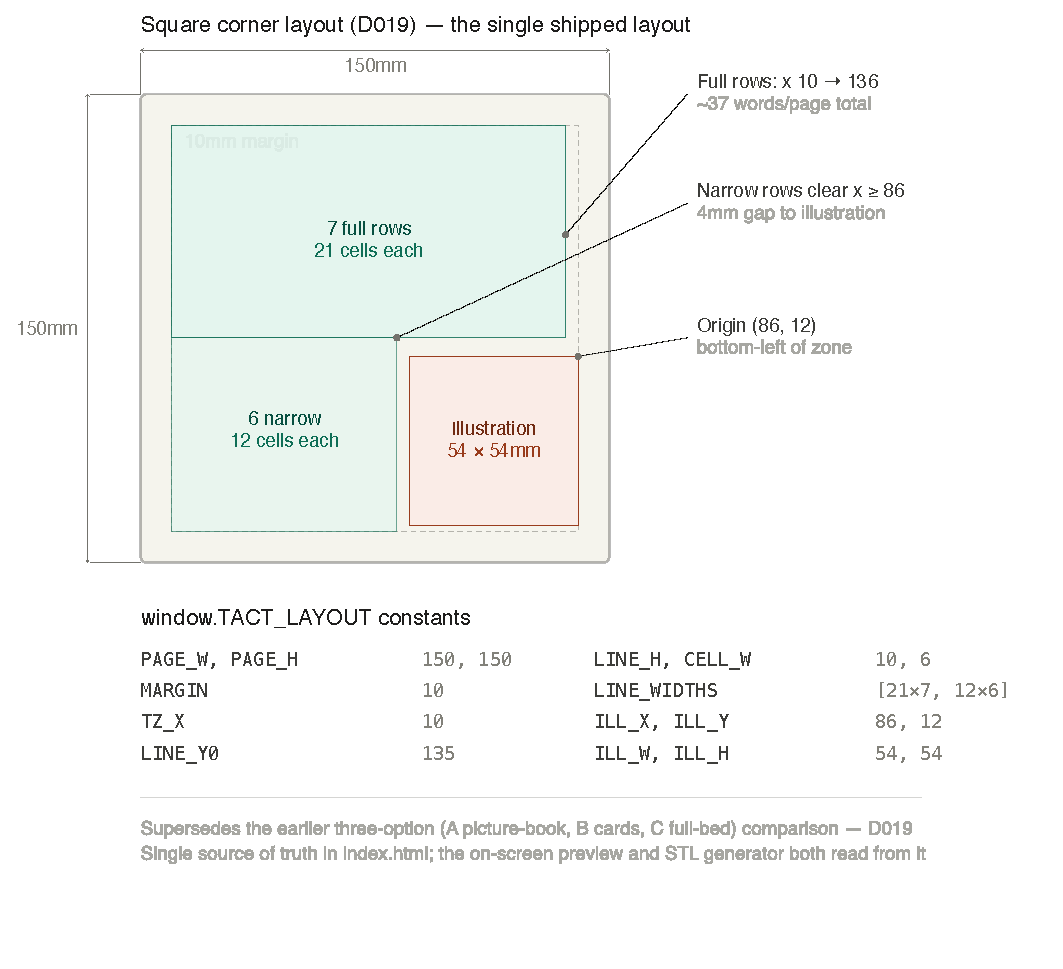
\includegraphics[width=0.85\textwidth]{tact_page_layout_geometry.pdf}
\caption{Dimensioned geometry of the shipped square corner layout. The 150 by 150 millimeter page carries a 10 millimeter margin, seven full Braille rows of 21 cells, six narrower rows of 12 cells that clear the illustration zone at $x \geq 86$, and a 54 by 54 millimeter illustration zone anchored at origin (86, 12). The coordinate constants shown are read directly by both the preview renderer and the STL exporter from one shared object, the mechanism that prevents the preview-print divergence described in Section~\ref{sec:layout}.}
\label{fig:geometry}
\end{figure*}

A second, independent bug surfaced once real multi-page stories were tested end to end. Pagination originally filled each page greedily, placing as many words as would physically fit before starting the next page, which meant a fifty-word story became a full 37-word first page followed by a nearly empty 13-word second page. A blind reader's fingers register a mostly blank page as unambiguously as sighted eyes do; it reads as broken, not as a stylistic choice. The first fix computed, for a given story, the fewest number of pages whose even split still fits every page, and distributed words accordingly.

That fix was later withdrawn, and the reasoning is worth recording because the intuition behind it is wrong in a way that is not obvious. Balancing does remove the near-empty final page, but it does so by moving the deficit backwards into pages that were previously full. Measured over identical stories, balancing eliminated all sparse final pages at the cost of leaving five of twelve intermediate pages incomplete. Since each page here is a separate physical card rather than a leaf in a bound book, the substitution is a poor one: it converts one visibly unfinished card into two, and an intermediate card has no illustration to occupy the space the text does not reach.

\subsection{Sizing Text to a Page That Cannot Be Resized}

An attempt was made to solve the problem upstream instead, by asking the language model for the number of words that exactly fills the available cards. This failed, and the measurements explain why. The window that fills two cards without spilling onto a third is narrow, approximately 63 to 70 words in Italian and 74 to 80 in English; the asymmetry is itself a Braille effect, since Italian words are longer and every capital letter consumes an additional cell for the capital indicator. Against a window of roughly $\pm5$ words, the model's output varied by approximately $\pm20$ words, and it saturated: constrained to seven sentences it would not exceed roughly 70 words regardless of the number requested. Successive prompt revisions moved conformity between 17 and 43 percent without converging, because no phrasing can make a model hit a target narrower than its own variance.

The problem was therefore moved out of the prompt and into the layout. Pages are filled greedily, so every page before the last is completely full, and the leftover collects on the final card, which is then given the illustration whenever the remaining text still fits the narrower L-shaped profile. The picture occupies the corner the words do not reach, and the card reads as composed rather than unfinished. A final card that is already full receives no illustration, because it does not need one. Under this scheme, measured across the same corpus, no card was left sparse without a picture, every page before the last was completely full, and 76 percent of stories fit two cards.

\subsection{Why Preview-Print Fidelity Is Not a Cosmetic Concern Here}

For a sighted user of ordinary creative software, a preview that is slightly off from the final output is an inconvenience. For this project, it is closer to a trust failure. The adult operating the printer on a blind child's behalf has no independent way to verify the physical result matches what they approved, beyond reading the same preview the child will eventually read by touch. The fix described above, one shared coordinate object driving both the screen and the STL file, exists specifically to make that trust structurally guaranteed rather than something requiring manual re-verification after every future change.

\section{Case Study: Tactile Illustration System}\label{sec:illustration}

\subsection{Illustration as a Second Literacy Channel, Not Decoration}

A raised picture beside a Braille passage is not ornamental in the way an illustration in a print book can be treated as ornamental. For a reader building a mental model of a story entirely through touch, a well-formed tactile shape is an additional, non-redundant channel of information. It can convey silhouette, posture, and identity in a way prose alone cannot, and a poorly formed one, an ambiguous blob, or a shape too fine-detailed to resolve by touch, actively confuses rather than helps. This is why the shape library uses hand-drawn, deliberately simplified line art rather than any form of automatically traced clip art or photograph outline, consistent with the general premise argued for tactile-graphic datasets in prior work \cite{tactilenet}.

\subsection{Construction Rules}

Every shape in the library follows fixed rules enforced across the entire set: strokes only, no fill, and closed paths wherever geometrically possible, since open paths risk producing non-manifold, unprintable geometry once extruded. No perspective or shading of any kind is permitted, and a hard cap on path complexity keeps the resulting three-dimensional geometry printable and the file size small. Each shape carries a short, structured metadata entry, category, descriptive tags, and natural size, cataloged in a machine-readable index alongside the corresponding Scalable Vector Graphics (SVG) file.

\subsection{A Frequency Study of Fairy-Tale and Bedtime-Story Subjects}

The initial shape library, built first, covered roughly 46 common categories: everyday animals, vehicles, basic nature and weather, simple buildings, generic human figures, and everyday objects. A deliberate gap analysis followed, consisting of a study of the subjects most frequently recurring across classic fairy tales and bedtime stories, drawing on the Brothers Grimm and Hans Christian Andersen tradition, Charles Perrault, Aesop, and the broader corpus of stories parents actually tell at bedtime, cross-referenced against what the existing library already covered. The gap was substantial and specific. There was no dragon, no unicorn, no fairy, no mermaid, no princess, no king, no queen, no witch, no wolf, no fox, no pig, no mouse, no sheep, no bee, no ladybird, and no snail. Separately, several existing entries were of noticeably lower craft than the rest of the set, most conspicuously the moon, which contained a modeling error causing a full circle and a crescent shape to render directly on top of one another, visually indistinguishable from a plain circle.

Two expansion passes followed, bringing the library to its current size of 89 hand-drawn shapes. The moon was rebuilt as a clean crescent with a simple sleepy face and an adjacent star, and the sun was given a small gentle face and cleaner rays. Both were brought in line with the visual quality of the library's best existing entries. The sitting cat, in particular, served throughout as the informal quality bar every new shape was measured against. The first expansion pass added dragon, unicorn, fairy, mermaid, princess, king, queen, witch, wolf, fox, pig, mouse, sheep, bee, ladybird, and snail, together with magic wand, sword, treasure chest, pumpkin, mushroom, teddy bear, and rainbow. The second pass added a further batch of high-frequency subjects surfaced by the same methodology: swan, deer, squirrel, hedgehog, snake, monkey, cow, knight, wizard, ghost, bell, lantern, candle, mirror, gift, balloon, ball, kite, snowflake, and bridge, bringing fairy-tale and bedtime-story coverage to a level the original 46-shape library could not have supported.

\subsection{From Substring Matching to Whole-Word Bilingual Matching}

Illustrations are chosen automatically by scanning a story's text for keywords, in both Italian and English, including plural and diminutive forms, for example \emph{lupo}, \emph{lupi}, and \emph{lupetto} against \emph{wolf} and \emph{wolves}. The first implementation matched keywords as substrings, which produced a specific, almost comic false-positive class. The Italian word for sea, \emph{mare}, contains the Italian word for king, \emph{re}, as a literal substring, so any story mentioning the sea incorrectly summoned a king illustration rather than anything related to water. The matcher was rewritten to tokenize story text into whole words and match against that word set exactly, which eliminates this entire category of error and was verified directly against a battery of test phrases in both languages before being shipped.

\subsection{From Vector Shape to Printable Relief}

At export time, the chosen illustration's SVG file is rasterized onto a small canvas sized to the illustration zone, preserving aspect ratio and centering the result so the shape is never stretched to fill a differently proportioned space. Each dark pixel becomes a small square pillar in the resulting three-dimensional mesh, raised to approximately 0.9 millimeters, slightly higher than the 0.85 millimeter Braille dots, specifically so a fingertip can distinguish illustration from text by height alone, without needing to consciously interpret the difference.

\section{Physical Fabrication}\label{sec:fabrication}

\subsection{Braille Dot Geometry}

All dot geometry follows ISO 17049:2013, the international standard for accessible design and the physical application of Braille on signage and equipment \cite{iso17049}, over-built by roughly 20 to 30 percent in every dimension to pre-compensate for a well-documented, consistent property of budget FDM printing: it under-produces small raised features relative to the design file. Table~\ref{tab:shrinkage} reports the designed dimensions against typically measured printed dimensions, and Fig.~\ref{fig:shrinkage} visualizes the same comparison.

\begin{table}[t]
\caption{Designed versus typically printed dot geometry on budget FDM printers.}
\label{tab:shrinkage}
\centering
\begin{tabular}{lrrr}
\toprule
Parameter & Designed & Printed & Change \\
\midrule
Dot diameter & 1.6 mm & 1.3 mm & $-19\%$ \\
Dot height & 0.85 mm & 0.60 mm & $-29\%$ \\
Cell spacing & 6.0 mm & 5.9 mm & $-2\%$ \\
Base plate thickness & 0.5 mm & 0.48 mm & $-4\%$ \\
\bottomrule
\end{tabular}
\end{table}

\begin{figure}[t]
\centering
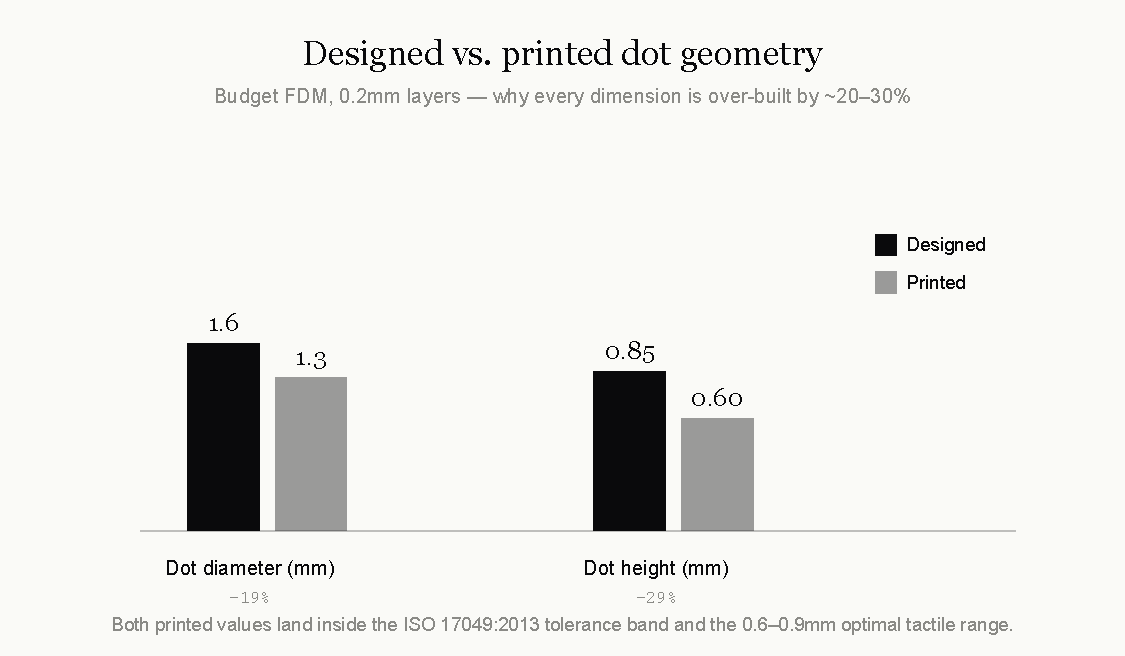
\includegraphics[width=\columnwidth]{chart-shrinkage.pdf}
\caption{Designed versus printed dot geometry on budget FDM printers. Both printed values land inside the ISO 17049:2013 tolerance band and the 0.6 to 0.9 millimeter range identified as optimal in blind-reader surveys, confirming that the 20 to 30 percent over-design correction is calibrated rather than arbitrary.}
\label{fig:shrinkage}
\end{figure}

Both printed values land inside the ISO tolerance band and inside the 0.6 to 0.9 millimeter range identified in blind-reader surveys as the optimal tactile dot height range; the over-design is a calibrated correction, not a guess. The dot profile itself combines a short cylindrical base with a hemispherical cap, rather than a pure hemisphere. A pure hemisphere at this diameter sits at the low end of the acceptable height range, and it prints with sharper curvature than budget FDM handles cleanly. The cylindrical base lifts the sphere's center of curvature instead, producing a rounder, gentler cap that is both more forgiving to print and more comfortable under a young fingertip. Every dot is rendered as sixteen-sided geometry, sufficient that no FDM printer could resolve additional smoothness, and no more, keeping file size and slicing time low. Fig.~\ref{fig:mockup} shows both the top-view page layout and this cross-section profile together, alongside the material and print settings used for the reference build.

\begin{figure*}[t]
\centering
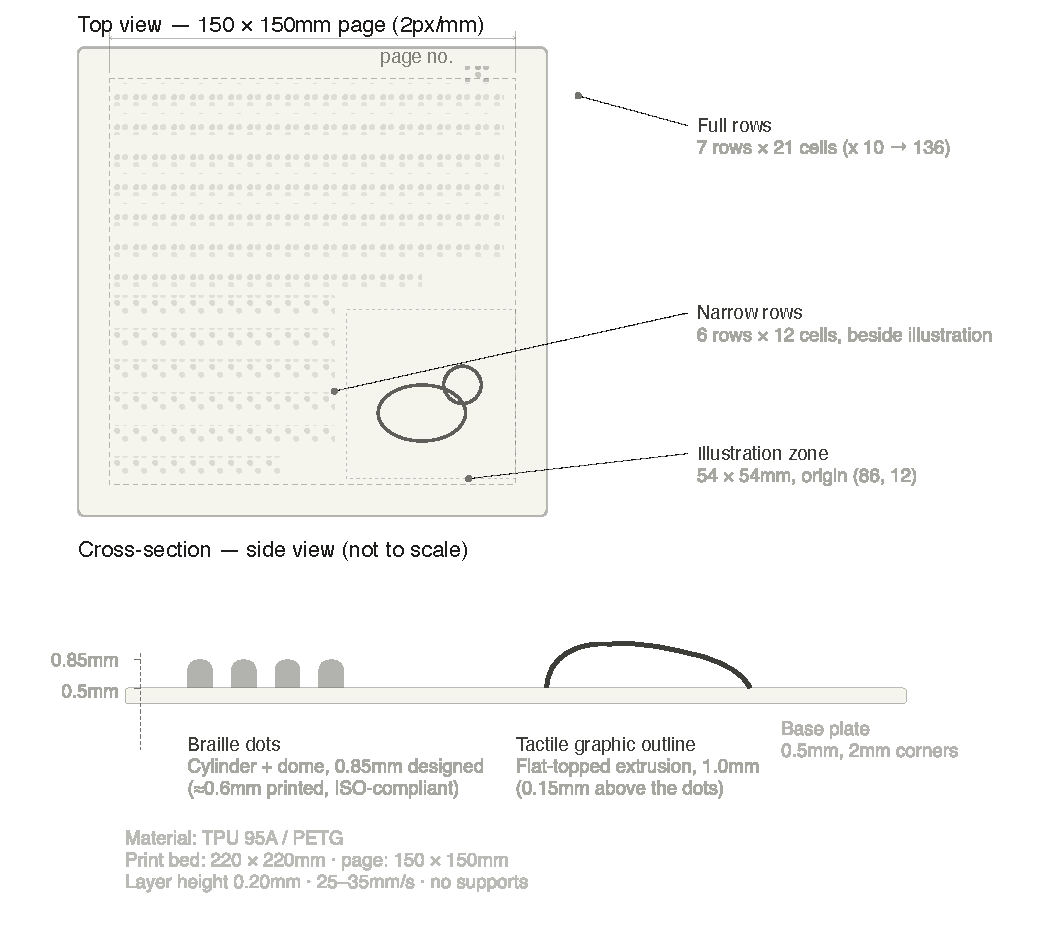
\includegraphics[width=0.85\textwidth]{tact_page_mockup.pdf}
\caption{Top view of the shipped 150 by 150 millimeter page (left) and a side-view cross-section (right, not to scale) comparing the domed Braille dot profile against the flat-topped tactile illustration extrusion. The cylinder-plus-dome Braille dot is designed to 0.85 millimeters and measures approximately 0.60 millimeters after FDM shrinkage, matching Table~\ref{tab:shrinkage}. The flat-topped illustration relief is extruded 0.15 millimeters higher, at 1.0 millimeters, so a fingertip distinguishes illustration from text by height alone, as discussed in Section~\ref{sec:illustration}.}
\label{fig:mockup}
\end{figure*}

\subsection{Base Plate and Separation Rules}

Every page sits on a continuous 0.5 millimeter base plate with 2 millimeter rounded corners, sized to survive routine handling without cracking. Separation distances are enforced structurally throughout, rather than checked case by case. Adjacent Braille cells maintain a 4.4 millimeter edge-to-edge gap, well within ISO tolerance. Tactile illustration pillars maintain a minimum 3 millimeter clearance from Braille text, and every printable element sits at least 5 millimeters from the page edge, guaranteed by the page margin.

\subsection{Material Guidance}

Table~\ref{tab:materials} summarizes material trade-offs across the four materials evaluated for this project.

\begin{table}[t]
\caption{Material trade-offs for printed pages.}
\label{tab:materials}
\centering
\begin{tabular}{lccl}
\toprule
Material & Flexibility & Durability & Role \\
\midrule
TPU 95A & High & Very high & Primary recommendation \\
PETG & Low & High & Rigid, washable alternative \\
PLA & None & Low & Excluded, too brittle \\
Recycled PET & Low--medium & High & Near-zero-cost option \\
\bottomrule
\end{tabular}
\end{table}

TPU 95A printed at approximately 220 degrees Celsius nozzle temperature and 50 degrees Celsius bed temperature, at a slow 25 to 35 millimeters per second for the cleanest possible dot definition and with no supports required, since the geometry is self-supporting by design, is the standard recommendation shipped with the project documentation.

\section{Interaction and Sound Design}\label{sec:sound}

\subsection{Why Sound Was Treated as a First-Class Design Surface}

A tool that leads with a microphone button and is explicitly meant to be usable by a screen-reader user cannot treat audio feedback as an afterthought layered on top of a visual interface. Every meaningful state change in the application, starting to listen, finishing listening, a story becoming ready, turning a page, downloading a file, has a corresponding sound, and every sound was deliberately composed rather than borrowed from a generic user-interface sound pack.

\subsection{Synthesis, Not Samples}

All audio is generated at runtime using the Web Audio application programming interface's oscillator and noise-buffer primitives \cite{w3cwebaudio}; there are no audio sample files anywhere in the project. This was a deliberate architectural choice consistent with the project's zero-dependency instincts elsewhere in the pipeline. Synthesized sound adds no download weight, works identically offline, and can be tuned with the same precision as the visual design tokens, rather than being limited to whatever a stock sample library happened to include. Every sound uses an exponential attack-and-release envelope rather than a linear one, which produces a soft, organic onset and decay instead of the harsher, clickier transient a linear ramp produces, a deliberately chosen detail, since abrupt sound transients are more likely to startle both young children and users with heightened auditory sensitivity.

\subsection{The Sonic Vocabulary}

Table~\ref{tab:sound} documents the full sonic vocabulary implemented in the shipped interface, together with the construction technique and design intent behind each sound.

\begin{table}[t]
\caption{The application's sonic vocabulary, construction, and design intent.}
\label{tab:sound}
\centering
\begin{tabular}{p{1.4cm}p{2.6cm}}
\toprule
Sound & Function and construction \\
\midrule
\texttt{listenStart} & Microphone activated. Two ascending sine chime pairs, C5+E5 then G5+B5. Rising pitch reads as an invitation to speak. \\
\texttt{listenEnd} & Microphone deactivated. A single tone falling into a two-note chime. Descending pitch reads as closure. \\
\texttt{ready} & Story finished generating. Three ascending chime steps forming a rising arpeggio, an unmistakable but unobtrusive completion cue. \\
\texttt{pageTurn} & Page navigation. A single very short, soft, low tone mimicking the tactile flick of a physical page. \\
\texttt{download} & File downloaded. A brief filtered noise burst plus a low chime, evoking paper and print texture. \\
\texttt{startLoader} & Model downloading or story generating. A slow two-tone pulse repeating roughly every 1.4 seconds, reading as a calm heartbeat rather than an anxious spinner. \\
\texttt{startPad} & Ambient background during longer waits. Three detuned sine oscillators with slow tremolo, low-pass filtered, a warm, non-sterile thinking texture. \\
\texttt{tap}, \texttt{toggle} & General interface confirmation. Short, quiet chimes, minimal and unobtrusive. \\
\texttt{type} & Keystroke feedback. A very short filtered noise burst, a subtle physical typing texture. \\
\bottomrule
\end{tabular}
\end{table}

All chime tones are pure sine waves, deliberately slightly detuned against each other within a single chord to add a gentle chorus-like warmth rather than sitting perfectly, sterilely in tune, and passed through a gentle low-pass filter to remove harsh upper harmonics. The entire sound system defaults to a conservative master gain and respects a persisted mute preference stored in the browser's local storage. Because browsers block audio from starting without a user gesture, the audio context is activated only on the visitor's first tap, keystroke, or touch, exactly as the platform requires.

\subsection{The Underlying Principle}

Nothing in the sonic vocabulary is arbitrary. Rising pitch consistently means beginning or anticipation. Falling pitch consistently means ending or resolution. An ascending multi-step arpeggio is reserved for the single moment of genuine payoff, the story becoming ready, so that moment is sonically distinct from routine navigation. Percussive, filtered noise is reserved specifically for physical actions with a real-world analog, typing and printing, rather than abstract interface events. A consistent sonic grammar, applied without exception across the whole interface, allows a user who is not looking at the screen to build an accurate mental model of what the application is doing, purely from what they hear. That is the entire point of treating sound as a first-class design surface rather than decoration.

\section{Visual and Typographic Design}\label{sec:visual}

The visual language is intentionally restrained: warm off-white paper tones rather than clinical white, a single near-black ink color used for essentially everything, and a deliberate typographic split into two distinct voices. A classic serif face is reserved for the story's own words and for the primary call-to-action headline, evoking a printed page rather than a software interface, while a monospaced, wide-letter-spaced uppercase face is reserved for interface chrome and status labels, page indicators, material specifications, and language toggles. This split gives the two kinds of content on the same screen, the story, which is the point, and the interface, which is merely the means, visibly different identities. The result screen deliberately mirrors the physical object it represents: a square card, subtly rotated and shadowed to read as a physical page rather than a flat interface panel. It shares the same dotted corner divider, the same illustration placement, and the same proportions the STL exporter will actually produce, directly reflecting the preview-print fidelity guarantee established in Section~\ref{sec:layout}.

\section{Representative Use Cases}\label{sec:usecases}

The system was designed against a spread of concrete scenarios, not a single idealized one, and each scenario below exercises a different combination of the requirements in Section~\ref{sec:requirements}.

\subsection{A Parent With a Capable Laptop}

WebGPU is available. The system downloads and caches a three-billion-parameter model on first use, writes a short sensory-rich story from a one-line spoken idea, and produces a two-page illustrated Braille book in well under a minute of active waiting.

\subsection{A Classroom on Older Hardware}

Older classroom Chromebooks frequently lack WebGPU support entirely. The teacher types, or a student dictates, a short story idea directly. No model is used at all. The words typed become the Braille text verbatim, matched to an illustration by keyword, and exported, a fully functional page with no download, no wait, and no degraded demonstration mode, directly exercising the graceful-degradation guarantee of Section~\ref{sec:llm}.

\subsection{A Deafblind Child Working With a Caregiver}

For this population, Braille is the only literacy channel available, and there is no audio fallback to lean on if any step of the pipeline were audio-dependent, which is why every step of the pipeline has a fully non-audio path from input through to the printed page.

\subsection{A Bilingual Household}

A household switching between Italian and English mid-session exercises every interface string, every Braille table, and every illustration keyword list in full for both languages, rather than one language being a partial or secondary translation of the other.

\subsection{A Rural or Low-Connectivity Setting}

Once opened, the application continues to function offline. Braille translation, illustration matching, layout, and STL export all run locally regardless of network state. Only story writing needs the network, and only for the hosted path; the in-browser model requires connectivity once, for its download, and none afterwards.

\subsection{An Older, More Independent Reader}

An older blind reader who prefers to type a request directly rather than use voice is served by the same text-input path as every other user, rather than a secondary, lesser-supported mode of interaction.

\section{Evaluation}\label{sec:evaluation}

\subsection{Verification Performed to Date}

The following checks were performed directly against the running application and are reported here as concrete, reproducible data points rather than as general assurances. Table~\ref{tab:verification} summarizes the results.

\begin{table}[t]
\caption{Engineering verification performed against the running application.}
\label{tab:verification}
\centering
\begin{tabular}{ll}
\toprule
Check & Result \\
\midrule
Braille round-trip decode (IT/EN) & Exact character match \\
STL byte-length validation & Matched expected size in all cases \\
Pagination of 200-word input & 10 pages of 20 words, 0 lost \\
Illustration keyword matching & Correct shape in all tested phrases \\
Console errors across full pipeline & None observed \\
\bottomrule
\end{tabular}
\end{table}

Braille fidelity was verified by decoding generated dot patterns programmatically back into text and comparing the result character by character against the original story, in both Italian and English, across multiple test passages. Every comparison confirmed exact agreement, with no silent mistranslation and no clipped content at page boundaries. Structural validity of every exported STL file was checked against the expected byte length for the binary format, an 80-byte header plus a 4-byte triangle count plus 50 bytes per triangle. This was tested for pages containing Braille only, illustration only, and both combined. One specifically illustrated example produced approximately 37{,}000 triangles at 150 by 150 millimeters, and the byte length matched the formula in every case tested. A synthetic input of 200 words was paginated and verified to split into ten pages of exactly twenty words each, with zero words lost, the specific failure mode a naive rebalancing implementation would risk. Cross-language shape selection was verified against a battery of Italian and English test phrases covering the full expanded shape library, including the substring false-positive case described in Section~\ref{sec:illustration}, and confirmed fixed. No unhandled runtime errors were observed across a full run of the pipeline: voice input, story generation both with and without a language model available, Braille translation, illustration matching, and STL export, all checked directly against the browser console on each pass.

\subsection{What This Evaluation Does and Does Not Establish}

This is engineering-level verification, not user research, and that distinction is stated explicitly rather than blurred. The checks above confirm the pipeline does what it was designed to do. They say nothing about whether the physical output is comfortable, legible, and enjoyable under a blind child's fingers, a question only real users can answer, and one this project has not yet asked them, a limitation revisited in Section~\ref{sec:limitations}.

\subsection{Comparison With Prior Systems}

Tact differs from the related systems in Section~\ref{sec:related} primarily in deployment cost and hardware assumption. TaleVision and TactileNet demonstrate that AI-assisted tactile content generation improves outcomes for blind children, but neither is an open, deployable end-user tool \cite{talevision,tactilenet}. AltCanvas and Chart4Blind both assume a human author, sighted or blind, actively composing a scene through a manual interface, whereas Tact composes the page automatically from a one-sentence prompt \cite{altcanvas,chart4blind}. BrailleRAP is the most directly comparable open hardware project \cite{braillerap}. Relative to it, FDM three-dimensional printing trades faster per-page embossing time for a page that survives repeated handling and for reliance on general-purpose hardware a household may already own. Relative to a purely cloud-hosted system, Tact keeps in-browser inference following the WebLLM architecture as a path that removes both the recurring cost and the data-transmission step \cite{webllm}, while placing a hosted path in front of it for speed. The price of the in-browser path is a one-time model download and a quality ceiling set by the reader's own hardware; the price of the hosted path is that one sentence leaves the device. Both are documented in Sections~\ref{sec:llm} and~\ref{sec:hosted}.

\section{The Zero-Cost Architecture in Full}\label{sec:zerocost}

Table~\ref{tab:zerocost} enumerates every pipeline step against its default technology and its cost, demonstrating that no step in the default path gates basic functionality behind a payment.

\begin{table}[t]
\caption{Cost of every pipeline step under the default configuration.}
\label{tab:zerocost}
\centering
\begin{tabular}{p{2.3cm}p{2.9cm}p{0.9cm}}
\toprule
Step & Default technology & Cost \\
\midrule
Speech input & Browser-native speech recognition & Free \\
Story writing & In-browser model, adaptive & Free \\
Writing fallback & The user's own words & Free \\
Braille translation & From-scratch Grade 1 table & Free \\
Illustration & Local shape library & Free \\
Layout \& export & Local computation & Free \\
Hosting & Static file, any host or none & Free \\
\bottomrule
\end{tabular}
\end{table}

A future, optional path for locally run larger models, for example through a tool such as Ollama, or a user-supplied API key for a commercial provider, remains architecturally possible within the original structured schema described in Section~\ref{sec:architecture}. It is documented explicitly as a future, opt-in upgrade for users who want it, never as a requirement for basic functionality.

\section{Ethical Considerations}\label{sec:ethics}

Three commitments run through every decision documented in this paper, stated here explicitly rather than left implicit in the engineering choices alone.

First, nothing about us without us: every design choice to date has been made without direct input from a blind or deafblind user, because that input has not yet been sought. This is treated as an open liability rather than a footnote, as established in Section~\ref{sec:population}.

Second, privacy by construction rather than by policy: because story generation runs on the reader's own device by default, there is no server-side log of what stories a family generates, what a child asked for, or when. This is a structural property of the architecture, not a promise that could later be quietly walked back.

Third, no dependency that can be discontinued out from under a family. A single static file, a permissive license, and a zero-cost default path together mean that a school or family adopting this tool is not exposed to a subscription that might lapse, a company that might shut down, or an account that might be deleted.

\section{Limitations and Future Work}\label{sec:limitations}

Several limitations are stated plainly here, without softening, because an honest account of what remains undone is as much a contribution of this paper as the engineering that has been completed.

No testing with blind or low-vision readers has occurred yet. Every claim in this paper about tactile legibility, dot comfort, and illustration clarity rests on published standards and survey data, not on direct observation of this project's own output in real hands. This is judged the single most important open item ahead of any claim of readiness. The Italian organizations this project intends to work with have not yet been contacted. Outreach to the Biblioteca Italiana per i Ciechi Regina Margherita, the Istituto dei Ciechi di Milano, UICI Lombardia, and Lega del Filo d'Oro remains to be initiated.

A locally installable command-line package does not yet exist. The browser application is fully functional on its own, but a package for batch generation, automation, and integration into existing school or library workflows remains future work. Double-sided, interpoint, printing is also deferred. Genuine interpoint Braille, in which dots on the front and back of a page are offset so they do not interfere with one another, is a solved problem on paper embossers but a meaningfully harder one in extruded three-dimensional geometry, and has not yet been attempted. Automated print-farm integration, for example through OctoPrint, is deferred in favor of the simpler, more universally compatible download-and-open-in-any-slicer path.

A manual model-selection interface does not yet exist. The adaptive tiering described in Section~\ref{sec:llm} is currently fully automatic. Giving a user the ability to explicitly choose a smaller model for speed, or a larger one on capable hardware, including the eight-billion-parameter tier currently reachable only programmatically, is a natural, low-risk next step, precisely because the underlying tier-list architecture already supports it. A two-pass draft-then-revise generation mode was considered as a way to further improve story quality, at the cost of roughly doubling generation time, and was deliberately deferred in favor of keeping the default experience fast.

\section{Conclusion}\label{sec:conclusion}

Braille literacy did not decline because Braille became a worse technology. It declined because the economics of producing Braille content never adjusted to match the economics of producing print content. A blind child's ability to ask for a story about the thing they are currently obsessed with, a dragon, a specific kind of boat, their own name, was quietly priced out of existence somewhere along the way. This paper's claim is narrow and falsifiable: the specific combination of browser-based language inference, a small deterministic Braille translator, a hand-built tactile illustration library, and consumer FDM three-dimensional printing is now mature and cheap enough to put that ability back within reach of an ordinary family. The only requirement is a 70 euro printer. Four pieces of engineering, documented across Sections~\ref{sec:llm} through~\ref{sec:illustration}, support this claim. A WebAssembly failure was diagnosed and replaced. An adaptive model tiering rule was built around a real false positive in the browser's own capability signals. A page geometry error was corrected after a preview silently diverged from the print, and a pagination scheme was rebalanced after a genuinely empty-looking page was caught. Together, they are offered as evidence that the claim has been tested rigorously at the systems level. The representative use cases in Section~\ref{sec:usecases} and the verification results in Section~\ref{sec:evaluation} confirm the pipeline is ready for that final step. What remains, and what this project treats as the actual finish line rather than this paper, is putting a printed page into a blind child's hands and finding out, from them, whether it was worth building at all.

\appendix

\section{Braille Cell Reference}

A standard Braille cell is a two-by-three grid of potential dot positions, numbered by convention with dots 1, 2, and 3 forming the left column, top to bottom, and dots 4, 5, and 6 forming the right column, top to bottom. Physical spacing used throughout this project, documented fully in Section~\ref{sec:fabrication}, places 2.5 millimeters between dot centers within a cell in both directions, 6.0 millimeters between the start of one cell and the next, and 10.0 millimeters between the baseline of one line of Braille and the next.

\section{Glossary}

Grade 1 Braille denotes uncontracted Braille, one cell per character, with no shorthand contractions, and is the standard for beginning readers and the only form Italian Braille has. Grade 2 Braille denotes contracted Braille, English only, using roughly 180 shorthand contractions, typically introduced after Grade 1 fluency. FDM denotes fused deposition modeling, the most common consumer three-dimensional printing process, in which molten plastic filament is extruded layer by layer. TPU and PETG denote flexible and rigid three-dimensional-printing filament materials, respectively. STL denotes a standard three-dimensional model file format understood by essentially every three-dimensional printer slicer application. WebGPU denotes a browser application programming interface providing direct, general-purpose access to a device's graphics hardware \cite{w3cwebgpu}.

\section*{Acknowledgment}

The author thanks Francesco Giuliani, whose independent reimplementation of this system \cite{tattodev} demonstrated that reaching a language model over the network, rather than downloading one into the browser, removes a barrier this project had underestimated. The hosted path described in Section~\ref{sec:hosted} exists because of that work. The two projects share no code and are developed independently.

\begin{thebibliography}{00}

\bibitem{iso17049} International Organization for Standardization, ``Accessible design, application of braille on signage, equipment and appliances,'' ISO 17049:2013, 2013.

\bibitem{ueb} International Council on English Braille, ``Rules of Unified English Braille,'' 2024.

\bibitem{liblouis} Liblouis Project, ``Liblouis: An open-source braille translator and back-translator.'' [Online]. Available: https://liblouis.io

\bibitem{braillerap} BrailleRAP Project, ``BrailleRAP: An open-source DIY braille embosser.'' [Online]. Available: https://www.braillerap.org/en/

\bibitem{nfb2024} National Federation of the Blind, ``Braille illiteracy crisis.'' [Online]. Available: https://nfb.org/braille-illiteracy-crisis

\bibitem{talevision} H. Wu, H. Yang, F. Chang, D. Zhu, and Z. Liu, ``AI-generated tactile graphics for visually impaired children: A usability study of a multimodal educational product,'' \emph{International Journal of Human-Computer Studies}, vol. 198, Art. 103474, 2025.

\bibitem{tactilenet} A. Khan, A. Choubineh, M. A. Shaaban, A. Akkasi, and M. Komeili, ``TactileNet: Bridging the accessibility gap with AI-generated tactile graphics for individuals with vision impairment,'' arXiv:2504.04722, 2025.

\bibitem{altcanvas} S. Lee, M. Kohga, S. Landau, S. O'Modhrain, and H. Subramonyam, ``AltCanvas: A tile-based editor for visual content creation with generative AI for blind or visually impaired people,'' in \emph{Proc. 26th Int. ACM SIGACCESS Conf. Computers and Accessibility}, 2024.

\bibitem{chart4blind} O. Moured, M. Baumgarten-Egemole, A. Roitberg, K. Muller, T. Schwarz, and R. Stiefelhagen, ``Chart4Blind: An intelligent interface for chart accessibility conversion,'' in \emph{Proc. 29th Int. Conf. Intelligent User Interfaces}, 2024.

\bibitem{webllm} C. F. Ruan \emph{et al.}, ``WebLLM: A high-performance in-browser LLM inference engine,'' arXiv:2412.15803, 2024.

\bibitem{w3cwebgpu} World Wide Web Consortium, ``WebGPU,'' W3C Candidate Recommendation Draft. [Online]. Available: https://www.w3.org/TR/webgpu/

\bibitem{w3cwebaudio} World Wide Web Consortium, ``Web Audio API,'' W3C Recommendation, 2021. [Online]. Available: https://www.w3.org/TR/webaudio-1.1/

\bibitem{tattodev} F. Giuliani, ``tatto.dev: a production reimplementation of Tact,'' 2026. [Online]. Available: https://github.com/francescogiuliani87/tatto.dev

\bibitem{agnes} Agnes AI, ``Agnes 2.0 Flash,'' model documentation. [Online]. Available: https://agnes-ai.com/en/docs/agnes-20-flash

\end{thebibliography}

\end{document}
